\section{Electrodiffusion in the extracellular space}
\label{sec:Eldiff}
\index{Electrodiffusion}
In the standard VC theory presented in Chapter \ref{sec:VC}), we assumed that extracellular currents, and thus extracellular potentials, are exclusively due to ohmic drift. However, when ion concentrations are present in the extracellular space, there will also be diffusive currents present, which can evoke so called diffusion potentials. 

In this chapter, we will introduce a more general, electrodiffusive theory for extracellular dynamics, which accounts effects of ionic diffusion as well as ohmic drift. However, before we present the electrodiffusive theory, we will try to get an intuition of how diffusion potentials arise.

\subsection{\blue{What is a diffusion potential?}}
\label{sec:Eldiff:LJpot}
\index{Diffusion potential}
We can get an intuitive understanding of what a diffusion potential is by considering a simple two-compartment system with two ionic solutions interacting at a junction  (Fig. \ref{Eldiff:fig:diffpot}). Let us assume that the left compartment contains a high concentration of NaCl, while the right compartment contains a lower concentration of NaCl (Fig. \ref{Eldiff:fig:diffpot}A). Initially, both compartments are electroneutral, i.e., they contain equal amounts of Na$^+$ and Cl$^-$. As no electrical forces are present, the initial system dynamics will be driven exclusively by diffusion. 

\begin{figure}[!ht]
\begin{center}
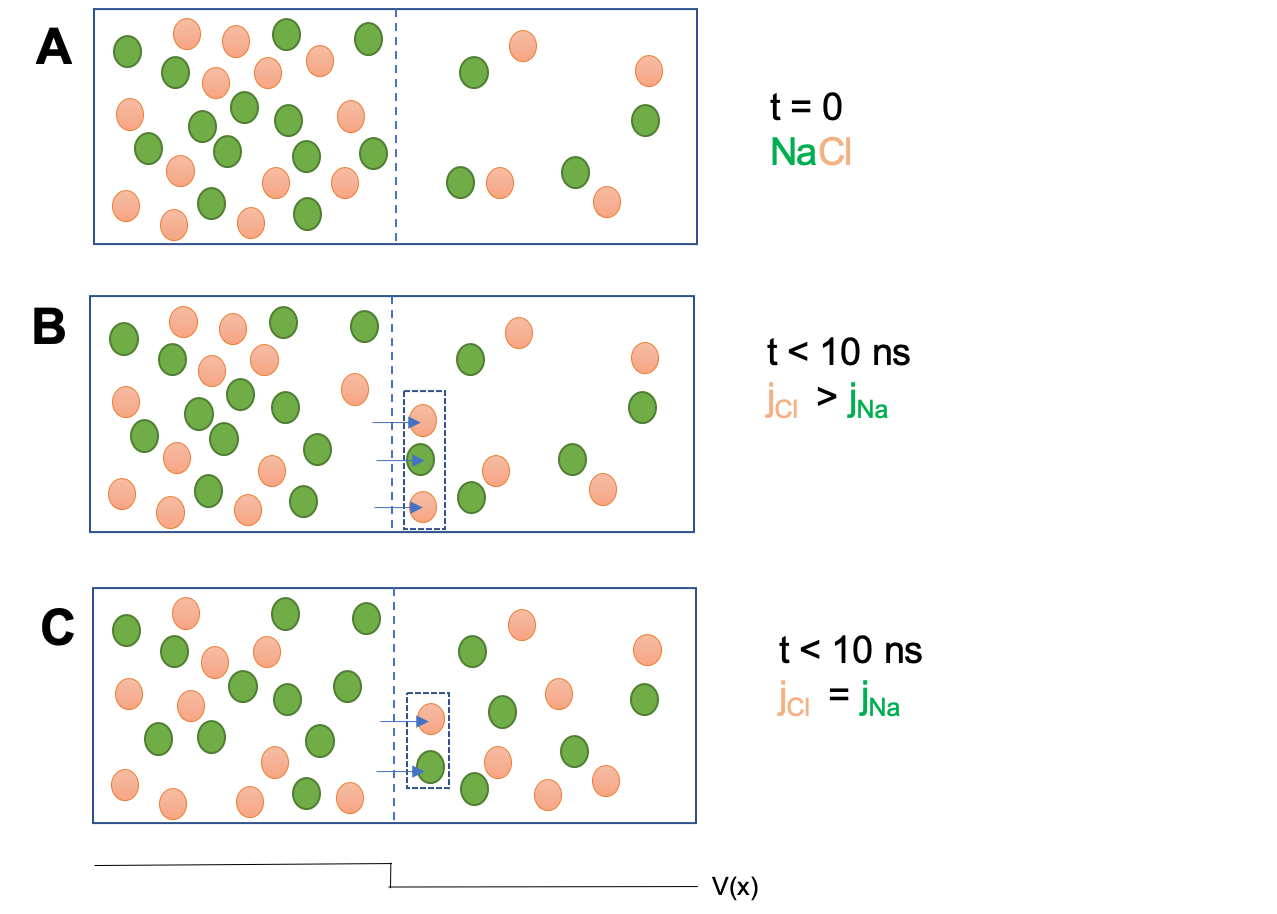
\includegraphics[width=0.8\textwidth]{Figures/Eldiff/Diffusionpot.png}
\end{center}
\caption{\textbf{Diffusion potential at the junction between two ionic solutions}. ({\bf A}) Initial condition with high concentration NaCl in the left compartment and low concentration NaCl in the right compartment. ({\bf B}) Since $D_{Cl} > D_{Na}$, we initially expect the flux of Cl$^-$ to be higher than the flux of Na$^+$. ({\bf C}) The net charge transfer in ({\bf B}) will give rise to a potential difference $\phi_d$ between the two compartments, which will prevent further charge accumulation. }
\label{Eldiff:fig:diffpot}
\end{figure}

Without solving any equations, we realize both Na$^+$ and Cl$^-$ will diffuse towards the low-concentration compartment on the right-hand-side. The diffusion speed for the various ions will be proportional to their respective diffusion constants, which in dilute solutions have the values given in Table \ref{Sigma:tab:diffconsts}). As the Table shows, the diffusion constant for Cl$^-$, is higher than that for Na$^+$. This means that rightward diffusive flux of Cl$^-$ will initially be larger than that for Na$^+$  (Fig. \ref{Eldiff:fig:diffpot}B). 

The fact that we initially have a higher diffusive flux of anions than of cations is quite dramatic. A charge-separation process like that will lead to an excess of positive charge in the left compartment and negative charge in the right compartment. In turn, this will give rise to a potential difference ($\Delta \phi_d$) between compartments. Since $\Delta \phi_d$ stems from a diffusion process, it is often called the diffusion potential. 

The diffusion potential will counteract the on-going charge separation process. That is, it will cause an electrical drift of anions (Cl$^-$) in the leftward direction, i.e., in the opposite direction from the diffusion of Cl$^-$. The net rightward flux of Cl$^-$ will therefore be reduced. Oppositely, it will cause a rightward drift of cations (Na$^+$), thus increasing the net rightward flux of Na$^+$. The effect of the diffusion potential is thus to reduce the Cl$^-$ flux and increase the Na$^+$ flux. Once it is gets big enough, $\Delta \phi_d$ will stabilize the system in a so-called quasi-steady state, where the net fluxes of Na$^+$ and Cl$^-$ have the same magnitude, and there will no longer will take place any net charge transfer (Fig. \ref{Eldiff:fig:diffpot}C). It has been shown that, in the extracellular medium of the brain, it only takes in the order of 10 ns to reach this quasi-steady state \citep{Solbra2018}. In the quasi-steady state, $\Delta \phi_d$ will still vary with time (hence the term "quasi"), but then at the much slower time-scale of ion concentration variations, which normally takes seconds to minutes.

To model the charge separation process taking place on a timescale, one need to run simulations with a sub-nanosecond time resolution, which is computationally demanding, and not even feasible for large systems. Fortunately, one can for many purposes obtain accurate predictions of both $\Delta \phi_d$ and ion concentration dynamics by using an electroneutral mathematical framework that does not model the charge relaxation process explicitly, but instead derives the quasi-steady state potential analytically under the assumption that it is reached instantaneously \citep{Solbra2018}. We shall introduce the modelling frameworks for electrodiffusive processes later on.

We note that the diffusion potential arises due to differences in diffusion constants between different ions present  (cf. Table \ref{Sigma:tab:diffconsts}). If all ions had identical diffusion constants, there would be no charge separation and thus no diffusion potential. We also note that the diffusion potential is not something very exotic and new for this chapter. The reversal potential of an ion channel (eq. \ref{Neuron:eq:revpots}) is essentially a single-ion diffusion potential, and the leakage reversal potential (eq. \ref{Neuron:eq:Eleak_GHK}) is a diffusion potential depending on the differences in passive membrane permeabilities (playing the role of diffusion constants) of the various ion species.

The diffusion potential is often called the liquid-junction potential, since it is most pronounced at the junction between to different ionic solutions \citep{Sokalski2001}. The liquid-junction potential ($\Delta \phi_{lj}$) is a familiar term for experimentalists performing patch clamp experiments. One then typically uses a pipette electrode filled with a ionic solution that resembles that of the intracellular medium. When the pipette pierces through brain tissue on its way to a target cell, it comes in contact with the extracellular solution. Through a process similar to that depicted in Fig. \ref{Eldiff:fig:diffpot}, only involving a larger number of different ions, a diffusion potential (with a typical magnitude of a few millivolts) is then instantly evoked at the junction between the pipette solution and the extracellular solution. This (roughly constant) potential difference over the pipette junction remains, and needs to be estimated and subtracted from the recordings of the cellular membrane potential.

Whereas the Nernst-Potential and liquid junction potentials in patch clamping are somewhat familiar examples of diffusion potentials, diffusion potentials in the extracellular space tend to be smaller in magnitude, and have not been that much studied in neuroscience. Below we will outline the physical theory for studying electrodiffusive processes, but before starting, we need to make some comments on the medium that we consider. 


\subsection{\blue{Continuous, porous medium approximation for electrodiffusion}}
\label{sec:Eldiff:porous}
\index{Continuous medium}
\index{Porous medium}
In Chapter \ref{sec:Sigma}, we introduced the continuous, porous medium approximation for coarse grained transports in brain tissue, and will use a similar approximation for electrodiffusive processes. However, unlike what we did in Chapter \ref{sec:Sigma}, where our reference volume was the tissue as a whole, we shall here follow the convention that we use only the fraction $\alpha$ of tissue that is extracellular space as our reference volume \citep{Nicholson2001}. All extracellular variables will then be defined relative to the actual volume that they exist in. The relevant variables, as defined through this convention, are: 

\begin{itemize}
\item $c_k$ (units $\mathrm{mol/m^3}$ = mM) will denote the extracellular concentration of an ion species $k$, defined as the number of extracellular ions of species $k$ (in mol) per extracellular volume unit (which is a fraction $\alpha$ of the tissue volume unit).

\item ${\bf j_k}$ (units $mol/\mathrm{m^2s}$) will denote the extracellular flux density of an ion species $k$, defined as the number of extracellular ions (in mols) per extracellular unit cross- section area (which is a fraction $\alpha$ of a unit tissue cross-section area) per second.

\item  ${\bf i_e}$ (units $\mathrm{A/m^2}$) will denote the extracellular current density, defined as extracellular current per per extracellular unit cross-section area. In comparison, the current density ${\bf i}$ in Chapter \ref{sec:VC} was defined as extracellular current per unit tissue cross-section area, which means that ${\bf i_e} = {\bf i}/\alpha$.

\item $\tilde{D}_k$ (units $\mathrm{m^2/s}$) will denote the effective diffusion constant \index{Diffusion constant} for ion species $k$ in the extracellular medium. It is defined so that the diffusive flux is given by ${\bf j_k^{diff}} = -\tilde{D}_k \nabla c_k$. The effective diffusion constant accounts for the fact that diffusing ions face obstacles (neurites) along their path forcing them take detours, reflected through a tortuosity $\lambda$ \citep{Nicholson1998}, and is given by:
\begin{equation}
\tilde{D_k} = \frac{D_k}{\lambda^2}, 
\label{Eldiff:eq:diffconst}
\end{equation}
where $D_k$ is the diffusion constant for an ion species $k$ in the pure (unhindered) extracellular solution. The fact that diffusing ions are confined the stay only in the extracellular volume fraction $\alpha$ is already accounted for in the flux definition.

\item $\sigma_e$ (units S/m) will denote the tissue averaged extracellular conductivity for extracellular current densities defined as ${\bf i_e}$. As we show later, $\sigma_e$ can be expressed as a function of ion concentrations:
\begin{equation}
\sigma_e = \frac{F}{\psi}\sum_{k} \tilde{D}_k z_{k}^2 c_{k}.
\label{Eldiff:eq:sigma1}
\end{equation}
Here $z_{k}$ is the valency of ion species $k$, and $\psi=RT/F$ is defined by the gas constant ($R$), Faraday's constant ($F$) and the temperature ($T$). Since $\sigma_e$ relates to ${\bf i_e}$ in the same way that $\sigma$ related to ${\bf i}$ in Chapter \ref{sec:VC}, $\sigma_e = \sigma /\alpha$.

\item $f_k$ (units mol/m$^3$) will represent the ion-flux-source density, i.e., the local neuronal output of an ion species $k$ per per extracellular volume unit. It is essentially is the ion-dynamics counterpart to the current-source-density (CSD) presented earlier (eq. \ref{VC:eq:CSD1}).

\item $C_e$ (units A/m$^3$) represents the current source density, i.e., the local neuronal output current per extracellular volume unit. $C_e = C/\alpha$ where $C$ (as defined in Chapter \ref{sec:VC}) is neuronal output current per tissue volume unit.

\end{itemize}


\subsection{\blue{Electrodiffusive ion concentration dynamics}}
\label{sec:Eldiff:ionconcentrationdynamics}
When modeling an electrodiffusive process, we keep track of the ion concentration dynamics of each individual ion species. With the effective diffusion constant, $\tilde{D}_k$, the flux density (${\bf j_k}$) of an ion species $k$ is given by the Nernst-Planck equation:
\begin{equation}
{\bf j_k} = - \tilde{D_k} {\bf \nabla} c_{k} - \frac{\tilde{D_k} z_k c_k}{\psi} {\bf \nabla} \phi.
\label{Eldiff:eq:JNP}
\end{equation}
The first term on the right hand side of eq. \ref{Eldiff:eq:JNP} is called Fick's law, which defines the ionic flux density due to diffusion $j_{k}^\text{diff}$. The second term is the additional drift flux density $j_{k}^\text{drift}$, which accounts for the flux density of ions moving along gradients in the extracellular potential $\phi$.

In eq. \ref{Eldiff:eq:JNP}, the the electrical mobility of the ions is $\tilde{D_k}/\psi$, and thus linearly related to their diffusion constant. This relationship is called the Einstein relation \index{Einstein relation}, and is valid for dilute solutions such as the extracellular fluid \citep{Grodzinsky2011}.

The general continuity equation for an ion species $k$ is,
\begin{equation}
\frac{\partial c_k}{\partial t} = - \nabla \cdot {\bf j_k} + f_k,
\label{Eldiff:eq:salamander}
\end{equation}
where we remember that all variables or parameters are defined relative to the extracellular unit volume or extracellular unit cross-section area. If we insert the electroduffusive flux density (eq. \ref{Eldiff:eq:JNP}) into eq. \ref{Eldiff:eq:salamander},
we get the Nernst-Planck continuity equation:
\begin{equation}
\frac{\partial c_k}{\partial t} = {\bf \nabla} \cdot \left[ \tilde{D_k} {\bf \nabla} c_k + \frac{\tilde{D_k} z_k c_k}{\psi} {\bf \nabla} \phi \right] + f_k.
\label{Eldiff:eq:NP}
\end{equation}

Before we explain how to solve the Nernst-Planck system of equations, we will in the next subsection show how they relate to to the VC theory presented in Chapter \ref{sec:VC}.


\subsection{\blue{Electrodiffusive electrodynamics}}
\label{sec:Eldiff:electrodynamics}
From the equations for ion concentration dynamics (eqns. \ref{Eldiff:eq:JNP}-\ref{Eldiff:eq:NP} ) we can derive a corresponding set of equations for net charge dynamics. If we multiply eq. \ref{Eldiff:eq:JNP} by $F\cdot z_k$ and sum over all ion species $k$, we get the extracellular current density:
\begin{equation}
{\bf i_e} = F\sum_k {z_k {\bf j_k}} = -\sum_k{F z_k \tilde{D_k}{\bf \nabla} c_{k}} - F\sum_{k} \frac{\tilde{D_k} z_{k}^2}{\psi}c_{k} {\bf \nabla}{\phi}, 
\label{Eldiff:eq:INPa}
\end{equation}
where the first term on the right hand side is the diffusive current density ${\bf i_e^\text{diff}}$, and the second term is the Ohmic drift current density ${\bf i_e^\text{drift}}$. Since we know from earlier that the drift current density should equal $- \sigma_e \nabla \phi$  (cf. eq. \ref{VC:eq:ohmici}) we may identify the the conductivity $\sigma_e$ of the extracellular medium as \citep{Koch1999}:
\begin{equation}
\sigma_e = \frac{F}{\psi}\sum_{k} \tilde{D}_k z_{k}^2 c_{k},
\label{Eldiff:eq:sigma}
\end{equation}
as we postulated in eq. \ref{Eldiff:eq:sigma1}. With this, we can write eq. \ref{Eldiff:eq:INPa} on the simpler form:
\begin{equation}
{\bf i_e} = - \sum_k{F z_k \tilde{D_k}{\bf \nabla} c_{k}} - \sigma_e{\bf \nabla}{\phi},
\label{Eldiff:eq:INP}
\end{equation}

Likewise, if we multiply eq. \ref{Eldiff:eq:salamander} by $F\cdot z_k$ and sum over all ion species, we get the continuity equation for charge: 
\begin{equation}
\frac{\partial \rho_e}{\partial t} =  \nabla \cdot \left (\sum_k{F z_k \tilde{D_k}{\bf \nabla} c_{k}} + \sigma_e\nabla\phi  \right)  + C_{ion}.
\label{Eldiff:eq:chargecontinuity}
\end{equation}
We have here introduced the extracellular charge density (define as extracellular charge per tissue unit volume), 
\begin{equation}
\rho_e = F \sum_k z_k c_k,  
\label{Eldiff:eq:roen}
\end{equation}
and the ionic current source, 
\begin{equation}
C_e^{ion} = F \sum_k z_k f_k. 
\label{Eldiff:eq:csden}
\end{equation}
The index "ion" signifies that this source term exclusively accounts for the sources $f_k$ mediated by ions that pass through the neuronal membrane and contributes to the extracellular ion concentration dynamics in eq. \ref{Eldiff:eq:NP}. Importantly, it is not identical to the total CSD, which contains an additional capacitive component, which represents the accumulation of a charge density $\rho_m$ (defined as charge per total tissue unit volume) at the outside of the neuronal membrane:
\begin{equation}
C_e = C_e^{ion} + C_e^{cap} = F \sum_k z_k f_k - \frac{\partial \rho_{mem}}{\partial t}.
\label{Eldiff:eq:CSDdecomposed}
\end{equation}
$C_e^{cap}$ interprets as the neuronal capacitive membrane current ($c_m \partial \phi_m/\partial t$) per extracellular unit volume, and the negative sign in front of the last term in \ref{Eldiff:eq:CSDdecomposed} follows from the fact that an outwards capacitive current (i.e., a source) implies an accumulation negative charge on the external side of the membrane. 

Let us now look at the charge density, $\rho_e$ at the left hand side of eq. \ref{Eldiff:eq:chargecontinuity}. In general, $\rho_e$ could be composed of free charges in the extracellular bulk solution as well as charges bound to the outside of the neural membrane, i.e., we could have $\rho_e = \rho_e^{free} + \rho_e^{mem}$. However, as we have argued earlier, the bulk solution is very close to electroneutral, and if we assume perfect bulk electroneutrality ($\rho_e^{free} = 0$), we must have that $\rho_e=\rho_e^{mem}$. We can then combine eq. \ref{Eldiff:eq:chargecontinuity}  with eq. \ref{Eldiff:eq:CSDdecomposed} to arrive at:

\begin{equation}
\nabla \cdot (\sigma_e\nabla\phi) = - C_e - F \nabla \cdot \left (\sum_k{z_k \tilde{D_k}{\bf \nabla} c_{k}} \right).
\label{Eldiff:eq:eldiffCSD2}
\end{equation}

Eq. \ref{Eldiff:eq:eldiffCSD2} is the electrodiffusive counterpart to eq. \ref{VC:eq:CSD2}, that we used as starting point in standard VC theory. For a more direct comparison, we can multiply eq.  \ref{Eldiff:eq:eldiffCSD2} with the extracellular volume fraction $\alpha$, and get:
\begin{equation}
\nabla \cdot (\sigma\nabla\phi) = - C - F\alpha \nabla \cdot \left (\sum_k{z_k \tilde{D_k}{\bf \nabla} c_{k}} \right).
\label{Eldiff:eq:eldiffCSD22}
\end{equation}
Comparing eq. \ref{Eldiff:eq:eldiffCSD22} and eq.  \ref{Eldiff:eq:eldiffCSD2}, we see that the difference between them is the last term in eq. \ref{Eldiff:eq:eldiffCSD22}, which is the diffusive contribution not accounted for in \ref{VC:eq:CSD2}. As eq. \ref{Eldiff:eq:eldiffCSD2} shows, also diffusive processes can contribute to the genesis of extracellular potentials, and if present, they could give rise to a non-zero $\phi$ even in the absence of neuronal sources ($C = 0$). Diffusive currents can thus be seen as an additional "source" for generating extracellular potentials \citep{Halnes2017}. 

We note that, apart from helping us realizing the relationship between standard VC theory and electrodiffusive theory, eq. \ref{Eldiff:eq:eldiffCSD2} is not very "user friendly". Whereas eq. \ref{VC:eq:CSD2} allows us to derive an analytical expression for the electrical potential at all points in space once the $C$ is known, eq. \ref{Eldiff:eq:eldiffCSD2} does not. To solve  eq. \ref{Eldiff:eq:eldiffCSD2}, we must keep track of the spatial distribution of ion concentrations by solving the Nernst-Planck system of equations (eq. \ref{Eldiff:eq:NP}) using some suitable numerical framework (see Chapter \ref{sec:Schemes}). 


\subsection{\blue{Do diffusion potentials matter?}}
\label{sec:Eldiff:estimates}
\index{Diffusion potential}
Due to the computational challenges they impose, it is tempting to make the assumption that diffusive currents contribute so little to the extracellular potential that we don't have to bother with them. This is what normally is being done, as most theoretical studies of extracellular potentials are based on standard VC theory. For most purposes, this is probably a good approximation, but its validity depends on one of the two following criteria being met:

\begin{enumerate}
\item C1: The magnitude of diffusive currents is much smaller than the magnitude of Ohmic drift currents.
\item C2: The frequency of diffusive currents is much smaller than the frequency of the CSD and the Ohmic drift currents. 
\end{enumerate}

The first criterion is general and quite intuitive. If C1 holds, the last term in eq. \ref{Eldiff:eq:eldiffCSD2} becomes much smaller than the other two terms, and standard VC theory will give accurate predictions of $\phi$. As we shall see below, it is quite likely that C1 is violated under many physiological conditions. If so, the second criterion (C2) may still come to our rescue. In most experiments, extracellular potentials are recorded using electrode systems with a lower cut-off frequency of 0.1-1 Hz \citep{Einevoll2007}. As diffusive currents are proportional to concentration gradients, which generally vary at a much slower time scale than $\phi$, diffusive contributions to $\phi$ are often direct-current (DC) like, i.e., they vary very slowly with time. If they vary slowly enough, they will not be picked up in recordings using standard electrode systems, only in experiments using DC electrodes. The question regarding their contribution to standard measurements is then whether they vary slowly enough. 

In the two following subsections we shall explore when and to which degree the criteria C1-C2 are likely to be met under physiological conditions.

\subsubsection{\blue{Magnitude of diffusion potentials.}}
Here, we will make some crude estimation of the magnitude that we can expect diffusion potentials to have in neural tissue. To make these, make the following simplifications of eq. \ref{Eldiff:eq:eldiffCSD2}): Firstly, diffusion potentials depend solely on extracellular concentration gradients, and not on the instantaneous activity of neurons. Let us therefore assume that $CSD = 0$, and consider the extracellular dynamics is governed by:
\begin{equation}
\nabla \cdot (\sigma_e\nabla\phi_d) = - \nabla \cdot \left (\sum_k{F z_k \tilde{D_k}{\bf \nabla} c_{k}} \right), 
\label{Eldiff:eq:eldiffCSD3}
\end{equation}
where we have denoted the potential $\phi_d$ since, in this case, it will exclusively be evoked by diffusion. Let us further consider a system with closed boundaries, so that no current can enter or leave the system. In that case, we may simply skip the first nabla, and take:
\begin{equation}
\sigma_e\nabla\phi_d = -\sum_k{F z_k \tilde{D_k}{\bf \nabla} c_{k}}, 
\label{Eldiff:eq:diffpot}
\end{equation}
Essentially, eq. \ref{Eldiff:eq:diffpot} states that the Ohmic drift current and diffusive current must cancel each others at each point in space, i.e., that if no current enters the system from the outside, no net current should be observed anywhere inside the system. The diffusion potential is thus the potential that we must have in the system for this to be the case. 

Finally, due to the linearity in eq. \ref{Eldiff:eq:diffpot}, the diffusion potential between two points in space is a direct function of the the ionic concentrations at these two points. Hence, it is sufficient for our task to consider a simple two-compartment system (like that in Fig. \ref{Eldiff:fig:diffpot}). For two-compartment systems, eq. \ref{Eldiff:eq:diffpot} further simplifies to:

\begin{equation}
\Delta \phi_d = \frac{F}{\bar{\sigma_e}} \sum_k{z_k \tilde{D}_k \Delta c_k}
\label{Eldiff:eq:diffpot2}
\end{equation}
where $\Delta c_k = c_{k}^{2} - c_{k}^{1}$ and $Delta \phi_d = \phi_d^{2} - \phi_d^{1}$ denote the concentration and potential difference between compartments 1 and 2. Within each compartment, $\sigma_e$ can be determined from the ionic concentrations by use of eq. \ref{Eldiff:eq:sigma1}. However, since we for this problem need the conductivity experienced by an Ohmic current traveling between the two compartments, we have in eq. \ref{Eldiff:eq:diffpot2} used the average $\sigma_e$ of the two compartments:
\begin{equation}
\sigma_e = \frac{F}{2\psi}\sum_{k} \left(\tilde{D}_k z_{k}^2 c_{k}^{1} + \tilde{D}_k z_{k}^2 c_{k}^{2} \right).
\label{Eldiff:eq:sigma2}
\end{equation}

Based on eq. \ref{Eldiff:eq:diffpot2}, we make some estimates of the magnitude of the diffusion potential for some test examples.

\begin{itemize}

\item {\bf Diffusion potential under spreading depression:} The most extreme extracellular concentration shifts in the brain occur under the pathological condition called spreading depression, where the extracellular K$^+$ concentration can change by several tens of millomolars. In an an example from hippocampus, the K$^+$ concentration was about 30 mM higher at the bottom hippocampal layer than at the top hippocampal layer (Fig. 1a in \citep{Herreras1993}). In that experiment, only K$^+$ concentrations were recorded. However, we may give a crude estimate of the diffusion potential between the top and bottom of hippocampus by making some simple assumptions of the other ion concentrations: (i) We assume that the top layer of hippocampus remained at baseline concentrations. In the experiment, this seemed to be close to the case for $c_K$ \citep{Herreras1993}. In the top layer, we may therefore assume some rather typical baseline concentrations with $c_{Na} = 150$ mM, $c_{K} = 3$ mM and $c_{Cl} = 153$ mM. (ii) In the bottom layer, we assume that the $c_K$ was 30 mM above baseline, and that the increase in $c_K$ was compensated by an identical decrease in $c_{Na}$, so that electroneutrality was preserved. A plausible mechanism behind this would be that all concentration shifts were due to neuronal AP firing, i.e., neurons exchanging Na$^+$ for K$^+$. With these assumptions, we have $c_{Na} = 120$ mM, $c_{K} = 33$ mM and $c_{Cl} = 153$ mM in the bottom layer. Plugging the top layer and bottom layer concentrations into eq. \ref{Eldiff:eq:diffpot2}, we obtain a diffusion potential $\Delta \phi_d \sim 1$ mV across the hippocampal depth.

\item {\bf Diffusion potential in cortex during neuronal hyperactivity:} In several experimental papers, extracellular concentration shifts of selected ions have been recorded during induced neuronal hyperactivity and seizure activity \citep{kriv1975, nicholson1978, Dietzel1982, somjen1986, Dietzel1989}. The main focus of these works are typically on $c_K$, which is the most critical extracellular concentration due to its low baseline value. In these experiments, $c_K$ can typically change from a baseline value around 3 mM up to a ceiling level between 8-12 mM before the dynamics becomes pathological and is driven into spreading depression. Dietzel et al. estimated the concentration shifts in both $c_{K}$, $c_{Na}$ and $c_{Cl}$, and cased on a series of recordings, they estimated that the maximal diffusion potential that could be expected under their experimental condition was 0.4 mV \citep{Dietzel1989}.

\item{\bf Diffusion potential during normal activity:} It is difficult to find experimental data that allows us to estimate diffusion potentials in the brain under "normal" conditions, and the question as to whether concentration gradients are present in a given brain region probably depends on the processing state it is in. However, recordings from anesthetized cat cortex have shown that even during the resting state, $c_K$ may exhibit small-amplitude (0.5 mM) fluctuations \citep{MCCREERY1983}. In experiments recording the response in cortex to moderate (not seizure inducing) stimuli applied in the thalamus, cortical $c_K$ increases were found to have a depth profile, and vary by about 2 mM between different cortical layers \citep{Cordingley1978}. Thus, it seems likely that there should be some concentration gradients present in neural systems, and that e.g., a concentration difference of about 1 mM between the top and bottom of cortex or hippocampus would not be unlikely under normal processing. If we repeat the calculation from spreading depression, but assume that $c_{K}$ and $c_{Na}$ in the bottom layer were increased/decreased by 1 mM instead of 30 mM, we get a diffusion potential of about $33 \mu$V. This is of the same magnitude as potentials typically recorded in LFP recordings. 

\end{itemize}

Based on the crude estimates above, it is likely that many experimental conditions can contain diffusion potentials of the same magnitude as the potentials recorded in extracellular recordings, such as the LFP. 


\subsubsection{\red{GH: Frequency of diffusion potentials}}
\ghnote{Krevende kapittel. Sammenligne noen powerspectra her. Regne ut et par selv, ala Gratiy.} 

Previous computational studies have predicted that effects of diffusion on extracellular potentials are not necessarily small, but tend to be very slow, meaning that they will only affect the very low-frequency components of $\phi$ \citep{Halnes2016, Halnes2017}. This is due to the diffusive current being a direct function of ion concentrations $c_k$, which on a large spatial scale typically vary on a much slower time scale (seconds-minutes) than the fluctuations in $\phi$ that we commonly are interested in (milliseconds-seconds). Furthermore, electrodes used to record $\phi$ typically have a lower cutoff frequency of 0.1-1Hz \citep{Einevoll2013}, which means that most of the tentative diffusive contribution will be filtered out from experimental recordings. It may therefore be a good approximation to neglect the diffusive term, except in the case of pathologically dramatic concentration variations.
